\documentclass[12pt,a4paper]{article}
\newcommand{\reportTitle}{Laboratory work 3:}
\newcommand{\reportSubject}{Study and Empirical Analysis of\\[0.3cm]DFS and BFS Graph Traversal Algorithms}
\usepackage{iftex}
\ifPDFTeX
    \usepackage[T1]{fontenc}
    \usepackage[utf8]{inputenc}
    \usepackage{mathptmx}
    \usepackage{courier}
\else
    \usepackage{fontspec}
    \setmainfont{Times New Roman}
    \setmonofont{Courier New}
\fi

\usepackage{amsmath}
\usepackage{graphicx}
\usepackage{float}
\usepackage[english]{babel}
\usepackage{indentfirst}
\usepackage{geometry}
\geometry{
    a4paper,
    left=20mm,
    right=10mm,
    top=20mm,
    bottom=20mm
}

\usepackage{setspace}
\setstretch{1.5}
\setlength{\parindent}{1.25cm}
\setlength{\parskip}{0pt}

\usepackage{titlesec}
\titleformat{\section}
  {\normalfont\bfseries\centering\fontsize{13}{15}\selectfont\MakeUppercase}{\thesection}{0.8em}{}
\titleformat{\subsection}
  {\normalfont\bfseries\fontsize{12}{14}\selectfont}{\thesubsection}{0.8em}{}
\titleformat{\subsubsection}
  {\normalfont\bfseries\fontsize{12}{14}\selectfont}{\thesubsubsection}{0.8em}{}

\titlespacing*{\section}{0pt}{0pt}{0.8\baselineskip}
\titlespacing*{\subsection}{0pt}{0.6\baselineskip}{0.3\baselineskip}
\titlespacing*{\subsubsection}{0pt}{0.4\baselineskip}{0.2\baselineskip}

\setcounter{secnumdepth}{3}

\usepackage{booktabs}
\usepackage{array}
\usepackage{longtable}
\usepackage{chngcntr}
\usepackage{caption}
\usepackage{subcaption}
\usepackage{enumitem}
\usepackage{needspace}
\usepackage{xcolor}
\usepackage{listings}
\usepackage{tocloft}

\setlist[itemize]{label=--,leftmargin=1.25cm,itemsep=0pt,topsep=0pt}
\setlist[enumerate]{leftmargin=1.25cm,itemsep=0pt,topsep=0pt}

\renewcommand{\cftsecleader}{\cftdotfill{1}}
\renewcommand{\cftsubsecleader}{\cftdotfill{1}}
\renewcommand{\cftsubsubsecleader}{\cftdotfill{1}}
\setlength{\cftbeforesecskip}{0pt}
\setlength{\cftbeforesubsecskip}{0pt}
\setlength{\cftbeforesubsubsecskip}{0pt}
\setlength{\cftsecindent}{0pt}
\setlength{\cftsubsecindent}{0.5cm}
\setlength{\cftsubsubsecindent}{1cm}
\setlength{\cftsecnumwidth}{1.0cm}
\setlength{\cftsubsecnumwidth}{1.0cm}
\setlength{\cftsubsubsecnumwidth}{1.2cm}
\renewcommand{\cftsecfont}{\bfseries}
\renewcommand{\cftsubsecfont}{\normalfont}
\renewcommand{\cftsecpagefont}{\bfseries}
\renewcommand{\cftsubsecpagefont}{\normalfont}
\renewcommand{\cfttoctitlefont}{\hfill\normalfont\Large\bfseries}
\renewcommand{\cftaftertoctitle}{\hfill}
\setcounter{tocdepth}{2}

\usepackage{hyperref}
\usepackage{bookmark}
\hypersetup{
    hidelinks,
    linktoc=all
}
\addto\captionsenglish{\renewcommand{\contentsname}{TABLE OF CONTENTS}}
\renewcommand{\contentsname}{TABLE OF CONTENTS}

\counterwithin{figure}{section}
\counterwithin{table}{section}
\counterwithin{equation}{section}

\newcommand{\reportcodestyle}{\linespread{1}\ttfamily\fontsize{10}{10}\selectfont}

\lstset{
    basicstyle=\reportcodestyle,
    frame=none,
    breaklines=true,
    columns=fullflexible,
    keepspaces=true,
    showstringspaces=false,
    aboveskip=0.2\baselineskip,
    belowskip=0.2\baselineskip
}

\captionsetup[figure]{
    font=bf,
    labelfont=bf,
    textfont=bf,
    labelsep=endash,
    justification=centering,
    singlelinecheck=false
}
\captionsetup[table]{
    font=normalfont,
    labelfont=normalfont,
    textfont=normalfont,
    labelsep=endash,
    justification=raggedleft,
    singlelinecheck=false,
    position=above
}

\newcommand{\studentName}{Ple\c{s}u Dinu}
\newcommand{\studentGroup}{FAF-241}
\newcommand{\teacherTitle}{asist. univ.}
\newcommand{\teacherName}{Fi\c{s}tic Cristofor}
\newcommand{\reportYear}{2026}
\newcommand{\reportCity}{Chi\c{s}in\u{a}u}

\newcommand{\makelabtitle}{
    \begin{titlepage}
        \centering

        \textbf{\large Ministerul Educa\c{t}iei \c{s}i Cercet\u{a}rii al Republicii Moldova}\\[0.3cm]
        \textbf{\large Universitatea Tehnic\u{a} a Moldovei}\\[0.3cm]
        \textbf{\large Facultatea Calculatoare, Informatic\u{a} \c{s}i Microelectronic\u{a}}\\[3cm]

        \vfill

        {\LARGE \reportTitle}\\[0.5cm]
        {\LARGE \reportSubject}\\[3cm]

        \vfill

        \begin{flushleft}
            \hspace{1cm}
            \begin{minipage}{0.8\textwidth}
                {\large Elaborated:}\\
                {\large st.\ gr.\ \studentGroup \hfill \studentName}\\[0.8cm]
                {\large Verified:}\\
                {\large \teacherTitle \hfill \teacherName}\\
            \end{minipage}
        \end{flushleft}

        \vfill

        {\large \reportCity\ - \reportYear}
    \end{titlepage}
}

\newcommand{\startreport}{
    \begin{document}
    \makelabtitle
    \newpage
    \pagenumbering{arabic}
    \setcounter{page}{2}
    \thispagestyle{empty}
    \tableofcontents
    \thispagestyle{empty}
    \newpage
}

\newcommand{\reportprelimsection}[1]{
    \newpage
    \section*{#1}
    \thispagestyle{empty}
    \phantomsection
    \addcontentsline{toc}{section}{#1}
}

\newcommand{\reportintroduction}{
    \newpage
    \section*{INTRODUCTION}
    \phantomsection
    \addcontentsline{toc}{section}{INTRODUCTION}
}

\newcommand{\reportmainsection}[1]{
    \newpage
    \section{#1}
}

\newcommand{\tocsubsection}[1]{
    \Needspace{12\baselineskip}
    \subsection{#1}
}

\newcommand{\reportlabel}[1]{
    \Needspace{6\baselineskip}
    \par\noindent\textbf{#1}\par
}

\newcommand{\reportfrontsubsection}[1]{
    \subsection*{#1}
    \phantomsection
    \addcontentsline{toc}{subsection}{#1}
}

\newcommand{\reportunnumberedsection}[1]{
    \newpage
    \section*{#1}
    \phantomsection
    \addcontentsline{toc}{section}{#1}
}

\newcommand{\reportreferences}[1]{
    \newpage
    \section*{REFERENCES}
    \phantomsection
    \addcontentsline{toc}{section}{REFERENCES}
    \begin{thebibliography}{99}
    #1
    \end{thebibliography}
}


\startreport

\reportprelimsection{LIST OF ABBREVIATIONS AND DEFINITIONS}
\begin{itemize}
    \item adjacency list -- graph representation in which each vertex stores the list of its neighboring vertices;
    \item BFS -- Breadth First Search, a graph traversal algorithm that visits vertices in order of their distance from the source, layer by layer;
    \item DFS -- Depth First Search, a graph traversal algorithm that follows each path as deeply as possible before backtracking;
    \item graph density -- the ratio between the number of existing edges and the maximum possible number of edges for a given vertex count;
    \item KB -- kilobytes, unit of memory measurement used throughout the benchmark;
    \item ms -- milliseconds, unit of time measurement used throughout the benchmark;
    \item traversal -- the systematic process of visiting all vertices reachable from a designated source vertex in a graph;
    \item visited set -- a data structure that tracks which vertices have already been discovered during a graph traversal.
\end{itemize}

\reportintroduction
Graph traversal is one of the most fundamental operations in computer science. Given a graph \(G = (V, E)\) and a source vertex, a traversal algorithm visits every vertex reachable from that source exactly once. The two classical traversal strategies are Depth First Search and Breadth First Search, and together they underlie a vast range of practical algorithms including connectivity analysis, cycle detection, topological sorting, shortest-path computation, and spanning tree construction.

Depth First Search explores the graph by following a single path as far as possible before retreating to explore alternative branches. The algorithm maintains an explicit stack, or equivalently uses the program call stack through recursion, to remember which vertices remain to be explored. Breadth First Search instead uses a queue to explore all vertices at the current depth before advancing to the next layer. This property makes BFS the method of choice whenever the shortest path in an unweighted graph is required, because the first time any vertex is reached is guaranteed to be via the shortest route.

Although both algorithms share the same asymptotic time complexity of \(O(V + E)\) on adjacency list representations, their concrete performance on a given computer depends heavily on graph density, graph topology, and the specific data structures chosen for the implementation. A set-based visited check has \(O(1)\) amortized cost per lookup, while a list-based check has \(O(n)\) worst-case cost, and this difference accumulates significantly on large or dense graphs. Similarly, a Python \texttt{deque} object supports \(O(1)\) popleft operations, whereas a plain list requires \(O(n)\) time to remove the first element. These implementation differences motivate a careful empirical study.

This laboratory work provides a systematic empirical comparison of DFS and BFS across graphs with different sizes, densities, and topologies. The study covers both a base implementation and an optimized implementation for each algorithm, allowing the effect of implementation choices to be isolated from the effect of graph structure. All experiments were conducted on directed and undirected graphs generated programmatically to ensure reproducibility.

\reportmainsection{ALGORITHM ANALYSIS}

\reportlabel{Objective}
Study and empirically analyze Depth First Search and Breadth First Search on graphs with varying vertex count, edge density, and topological structure, comparing execution time and peak memory usage between base and optimized implementation variants.

\reportlabel{Tasks}
\begin{enumerate}[leftmargin=1.25cm]
    \item implement DFS and BFS in both a base form and an optimized form in Python;
    \item establish the properties of the input data used for the analysis, including graph size, fill percentage, and named topology;
    \item select appropriate metrics for comparing the algorithms;
    \item perform empirical benchmarking of all four algorithm variants across all input sets;
    \item generate graphical representations of the obtained data;
    \item formulate conclusions based on the experimental results.
\end{enumerate}

\reportlabel{Theoretical Notes}
An alternative to mathematical analysis of algorithmic complexity is empirical analysis. Empirical analysis is useful when a preliminary estimate of the complexity class is needed, when two or more algorithms solving the same problem must be compared in practice, or when the practical effect of implementation details on a specific computing environment must be quantified \cite{gfg-bfs,gfg-dfs}.

A graph \(G = (V, E)\) consists of a set of vertices \(V\) and a set of directed or undirected edges \(E\). The two most common graph representations are the adjacency matrix and the adjacency list. The adjacency matrix stores a \(|V| \times |V|\) boolean or weight matrix and requires \(O(V^2)\) space regardless of the number of edges, while iteration over all neighbors of a vertex costs \(O(V)\). The adjacency list stores, for each vertex, only the list of its neighbors, requiring \(O(V + E)\) space and allowing neighbor iteration in \(O(\deg(v))\) time. Both DFS and BFS are defined for adjacency list representations, and their time complexity of \(O(V + E)\) is derived from the fact that each vertex and each edge is processed at most a constant number of times \cite{gfg-dfs,gfg-bfs}.

Depth First Search starts at the source vertex, marks it as visited, and then recursively or iteratively explores each unvisited neighbor in order. The iterative implementation maintains an explicit stack. When a vertex is popped from the stack, its unvisited neighbors are pushed onto the stack for future exploration. Because the stack follows a last-in first-out order, DFS always advances along the most recently discovered path before backtracking. The maximum stack depth at any point is bounded by the longest path explored so far, which in the worst case (a path graph) equals \(V - 1\). The memory requirement is \(O(V)\) for the stack and the visited structure combined. DFS terminates when the stack is empty, guaranteeing that all reachable vertices have been visited \cite{gfg-dfs,yt}.

Breadth First Search starts at the source vertex, marks it as visited, and enqueues it. While the queue is non-empty, the algorithm dequeues the front vertex and enqueues all its unvisited neighbors, marking them as visited at the moment of enqueueing, not dequeuing. This prevents the same vertex from being enqueued more than once. Because the queue follows a first-in first-out order, BFS always processes all vertices at distance \(d\) from the source before processing any vertex at distance \(d+1\). The maximum queue size at any point is bounded by the width of the graph's BFS tree, which on dense graphs can be large. The memory requirement is \(O(V)\) for the queue and the visited structure \cite{gfg-bfs}.

The key practical difference between DFS and BFS lies in their access patterns and memory footprint. DFS is biased toward depth: it can reach the far end of the graph very quickly but may delay visiting nearby vertices. BFS is biased toward breadth: it guarantees that the closest vertices are visited first but may accumulate many entries in the queue when the graph has high degree. On a complete graph with \(n\) vertices, BFS must enqueue all \(n - 1\) neighbors of the source before processing any of them, resulting in a queue of size \(n - 1\) after the first step. DFS would instead push all \(n - 1\) neighbors onto the stack in the same situation, producing an identical worst-case stack size. The empirical memory difference between the two therefore arises from the order in which entries are consumed: the DFS stack can accumulate multiple layers of unprocessed neighbors while still exploring a deep branch, while the BFS queue at each step contains only one frontier layer.

\reportlabel{Comparison Metric}
The following metrics were selected for the empirical comparison:
\begin{itemize}[leftmargin=1.25cm]
    \item execution time in milliseconds, measured using Python's \texttt{time.perf\_counter} function, which provides sub-millisecond resolution independent of wall-clock time;
    \item peak memory usage in kilobytes, measured using Python's \texttt{tracemalloc} module, which tracks all heap allocations made during the execution of the traversal function;
    \item number of visited vertices, recorded at the end of each run to confirm correctness;
    \item execution success status, flagging any runs that terminated with an error.
\end{itemize}

Each configuration was executed multiple times and the median values were used in the analysis. The median is preferred over the mean because it is resistant to outliers caused by operating system scheduling and garbage collection pauses.

\reportlabel{Input Format}
Two complementary classification strategies for graph generation were used in order to study different aspects of algorithm behavior.

The first strategy classifies graphs by fill percentage, defined as the ratio of existing edges to the maximum possible number of edges \(n(n-1)\) for a directed graph or \(\frac{n(n-1)}{2}\) for an undirected graph. Fill values ranged from \(0\%\) to \(100\%\) in increments of \(10\%\). Vertex counts of 10, 50, 100, and 200 were used for the base variants. This strategy allows the effect of density to be studied in isolation while vertex count is kept constant.

The second strategy classifies graphs by named topology. The following graph types were generated and tested at sizes up to 1000 vertices:
\begin{itemize}[leftmargin=1.25cm]
    \item simple random graph -- edges assigned uniformly at random;
    \item dense graph -- edge probability \(0.65\) or higher;
    \item tree -- exactly \(n - 1\) edges forming a connected acyclic structure;
    \item cyclic graph -- a single directed or undirected cycle through all vertices;
    \item bipartite graph -- vertices split into two groups, edges only between groups;
    \item complete graph -- all \(\frac{n(n-1)}{2}\) possible undirected edges present;
    \item wheel graph -- one central hub connected to all outer vertices in a ring;
    \item grid-planar graph -- vertices arranged in a two-dimensional grid, edges to horizontal and vertical neighbors;
    \item weighted graph -- random topology with real-valued edge weights;
    \item disconnected graph -- two or more isolated components.
\end{itemize}

The topology-based approach allows the structural properties of a graph to be directly linked to algorithm behavior, revealing which topologies are inexpensive to traverse and which impose the greatest cost.

\reportmainsection{IMPLEMENTATION}

\tocsubsection{Depth First Search}

Depth First Search is the oldest and most widely applied graph traversal strategy. Its depth-first exploration order is naturally suited to problems that require a complete path to be identified, such as maze solving, topological ordering of directed acyclic graphs, detection of back edges in cycle detection, and the construction of DFS spanning trees. The iterative form presented in this laboratory is preferred over the recursive form for large graphs, because the recursive version is subject to Python's default recursion limit of one thousand calls, which can be exceeded on sparse deep graphs with hundreds of vertices.

\reportlabel{Algorithm Description}

The iterative DFS method uses an explicit stack to simulate the call stack of the recursive formulation. The algorithm is presented in the pseudocode below.

\begin{lstlisting}
DFS(graph, start):
    visited = empty set
    stack   = [start]
    while stack is not empty:
        node = pop from stack
        if node not in visited:
            add node to visited
            for each neighbor of node:
                if neighbor not in visited:
                    push neighbor onto stack
    return visited
\end{lstlisting}

The vertex is marked as visited when it is popped from the stack rather than when it is pushed. This is important because a vertex may be pushed multiple times if multiple of its predecessors in the DFS tree are processed in a single iteration, but the visited check ensures it is actually processed at most once. Each vertex is popped at most once, and for each popped vertex all its neighbors are inspected once, giving a total cost of \(O(V + E)\). The stack size is bounded by the number of vertices, giving \(O(V)\) space complexity.

In an undirected graph, each edge \((u, v)\) may cause \(v\) to be pushed onto the stack when \(u\) is processed, and \(u\) to be pushed when \(v\) is processed, but the visited check prevents either from being processed more than once. In a directed graph, each edge is examined exactly once in the direction it is defined.

\reportlabel{Implementation}

Two DFS variants were implemented for the benchmark. The base variant represents a straightforward implementation: the visited container is a Python list, and membership is checked using the \texttt{in} operator, which scans the list linearly. The stack is also a Python list, using \texttt{append} for push and \texttt{pop()} for pop, both of which are \(O(1)\) amortized.

The optimized variant replaces the list-based visited container with a Python \texttt{set}. Set membership tests in Python use a hash table internally and cost \(O(1)\) amortized, compared with the \(O(n)\) worst-case cost of a list scan. On a graph with 200 vertices at 50\% fill, the visited list can grow to 200 entries, meaning that on average 100 comparisons are required per membership check. With 200 vertices and roughly 10000 neighbor inspections on a dense graph, the total overhead from list-based visited checks is approximately one million comparisons, while the set-based variant reduces this to a negligible constant per check. The adjacency representation used is a Python \texttt{dict} of \texttt{list} objects, one entry per vertex \cite{repo}.

\reportlabel{Results}

The representative results for both DFS variants at \(50\%\) fill density, along with the corresponding BFS results for direct comparison, are presented in Table~\ref{tab:lab3-density}.

\begin{table}[H]
    \caption{DFS and BFS base results at 50\% density fill}
    \label{tab:lab3-density}
    \centering
    {\fontsize{11}{11}\selectfont\renewcommand{\arraystretch}{1}\begin{tabular}{llll}
\toprule
Algorithm & Nodes & Time (ms) & Memory (KB) \\
\midrule
BFS\_Base & 10 & 0.029 & 0.60 \\
BFS\_Base & 50 & 0.288 & 1.32 \\
BFS\_Base & 100 & 2.750 & 2.41 \\
BFS\_Base & 200 & 35.760 & 4.29 \\
DFS\_Base & 10 & 0.044 & 0.77 \\
DFS\_Base & 50 & 0.453 & 6.45 \\
DFS\_Base & 100 & 4.742 & 22.08 \\
DFS\_Base & 200 & 30.207 & 86.64 \\
\bottomrule
\end{tabular}
}
\end{table}

According to Table~\ref{tab:lab3-density}, execution time and memory usage both grow with vertex count for all variants. DFS at 200 nodes recorded a median execution time of \(30.207\) ms and a peak memory of \(86.64\) KB, compared with BFS at the same size, which recorded \(35.760\) ms and only \(4.29\) KB. The time values are comparable between the two algorithms at this density, but the memory difference is more than twenty-fold. This is consistent with the theoretical expectation: both algorithms visit the same vertices, but DFS accumulates neighbors on the stack over multiple unexplored branches simultaneously, while BFS limits the queue to the current frontier layer.

The scaling behavior of DFS execution time as a function of node count is presented in Figure~\ref{fig:dfs-nodes}.

\begin{figure}[H]
    \centering
    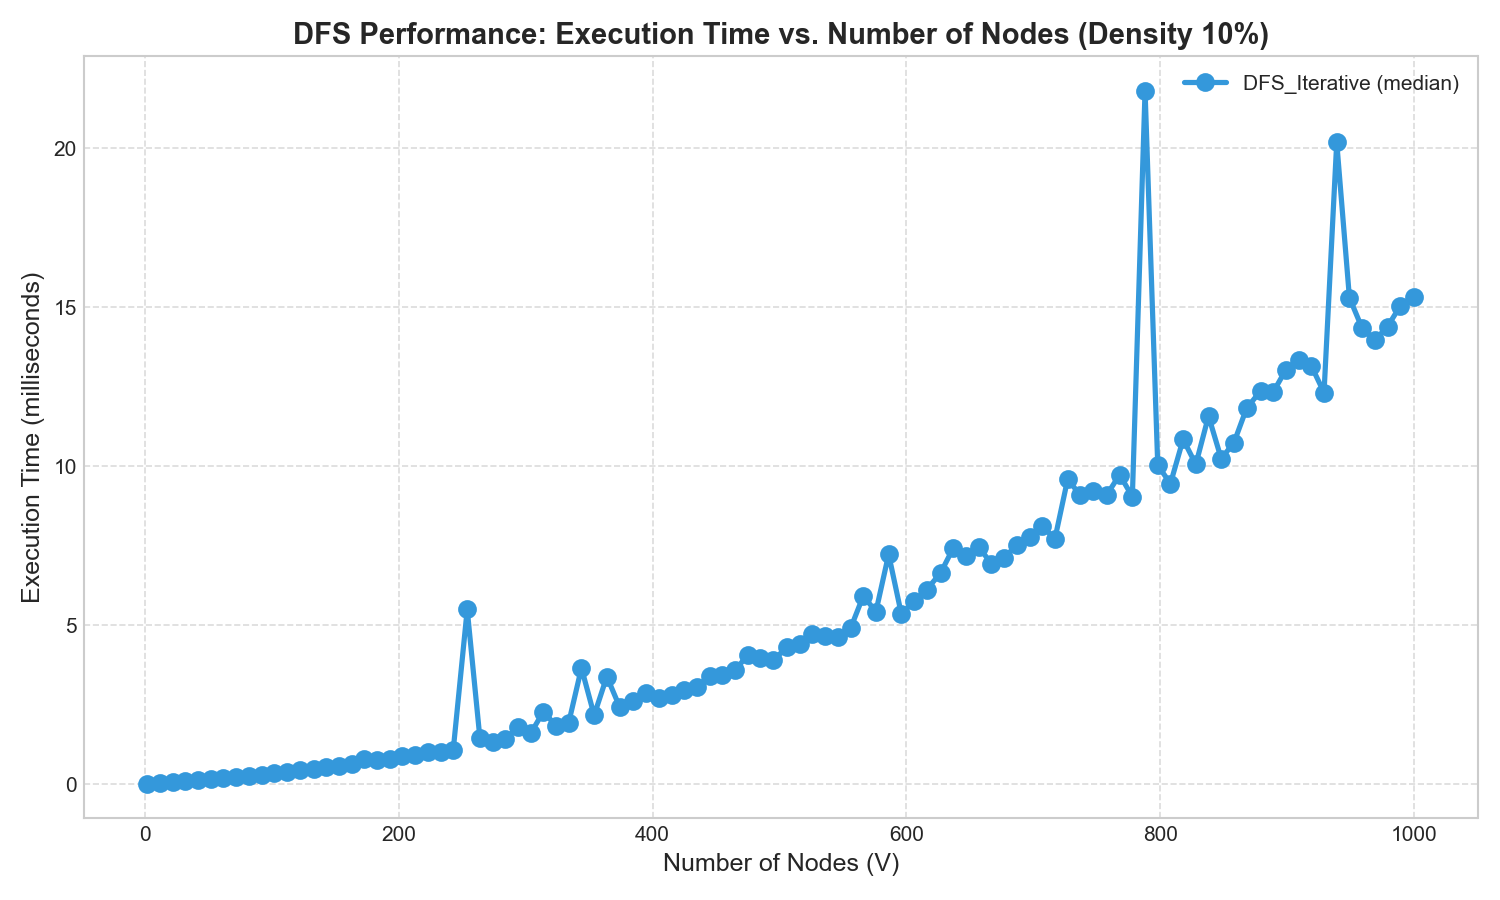
\includegraphics[width=0.83\textwidth]{../../Lab3/plots/dfs_performance_vs_nodes.png}
    \caption{DFS execution time as a function of node count}
    \label{fig:dfs-nodes}
\end{figure}

According to Figure~\ref{fig:dfs-nodes}, execution time grows consistently as the number of nodes increases. The slope is steeper for configurations with a higher fill percentage because a larger number of edges is processed per vertex. The base variant is slower than the optimized variant at all tested sizes, with the gap widening as the graph grows and the list-based visited check becomes increasingly expensive. The data confirms the \(O(V + E)\) behavior: when both vertex count and edge count grow (as they do when fill is held constant and node count is increased), the total work grows proportionally to the product of the two.

\reportlabel{Conclusion}

DFS performs as expected on all tested configurations. Its time complexity of \(O(V + E)\) is confirmed empirically, and the effect of the visited data structure on execution speed is clearly measurable. The iterative form is robust and avoids the recursion limit problem that would arise in the recursive version for graphs with a large number of vertices. The most significant practical finding is that DFS requires substantially more memory than BFS on dense graphs, which is a consequence of its stack-based exploration strategy accumulating many pending neighbors simultaneously.

\tocsubsection{Breadth First Search}

Breadth First Search visits vertices in non-decreasing order of their distance from the source. All vertices at distance one are visited before any vertex at distance two, all vertices at distance two are visited before any at distance three, and so on. This level-by-level order makes BFS the natural algorithm for computing shortest paths in unweighted graphs, for testing graph bipartiteness, and for building spanning trees that minimize depth. The level structure also makes BFS useful for problems where the proximity to a source determines processing priority, such as spreading simulations, network broadcast problems, and state-space search.

\reportlabel{Algorithm Description}

The BFS method uses a queue to maintain the exploration frontier. The algorithm is presented in the pseudocode below.

\begin{lstlisting}
BFS(graph, start):
    visited = {start}
    queue   = deque([start])
    while queue is not empty:
        node = popleft from queue
        for each neighbor of node:
            if neighbor not in visited:
                add neighbor to visited
                append neighbor to right of queue
    return visited
\end{lstlisting}

Crucially, a vertex is added to the visited set at the moment it is enqueued, not at the moment it is dequeued. This distinction ensures that each vertex is enqueued at most once, even if it is a neighbor of multiple already-processed vertices. Without this invariant, BFS would degenerate to \(O(E^2)\) complexity in the worst case because the same vertex could be enqueued multiple times. Each vertex is processed at most once and each edge is examined at most twice (once for each endpoint in an undirected graph), giving \(O(V + E)\) time complexity. Space complexity is \(O(V)\) for the queue and the visited set.

\reportlabel{Implementation}

The base BFS variant uses a Python list as the queue, calling \texttt{append} for enqueue and \texttt{pop(0)} for dequeue. The \texttt{pop(0)} operation shifts all remaining elements left by one position, which costs \(O(n)\) time, where \(n\) is the current queue size. On a graph where many vertices are on the same BFS level, this operation can dominate the total running time.

The optimized BFS variant uses Python's \texttt{collections.deque}, which is implemented as a doubly-linked list of fixed-size blocks and supports \(O(1)\) amortized \texttt{append} (right end) and \texttt{popleft} (left end) operations. The visited container is a \texttt{set} for \(O(1)\) amortized membership tests, identical to the optimized DFS variant. Together these two changes eliminate the quadratic cost incurred by the list-based variant on graphs with large frontier layers \cite{repo}.

\reportlabel{Results}

The optimized topology benchmark produced the most informative BFS results because different graph topologies expose fundamentally different traversal patterns. The representative values for the optimized BFS and DFS topology variants at 1000 nodes are presented in Table~\ref{tab:lab3-topology}.

\begin{table}[H]
    \caption{Optimized topology results at 1000 nodes}
    \label{tab:lab3-topology}
    \centering
    {\fontsize{11}{11}\selectfont\renewcommand{\arraystretch}{1}\begin{tabular}{lllll}
\toprule
Graph type & Algorithm & Median time (ms) & Median memory (KB) & Edges \\
\midrule
bipartite\_graph & BFS\_Optimized & 13.490 & 48.57 & 75187.0 \\
bipartite\_graph & DFS\_Optimized & 41.326 & 659.13 & 75187.0 \\
complete\_graph & BFS\_Optimized & 96.790 & 49.60 & 499500.0 \\
complete\_graph & DFS\_Optimized & 224.583 & 4110.82 & 499500.0 \\
grid\_planar & BFS\_Optimized & 1.680 & 44.20 & 1936.0 \\
grid\_planar & DFS\_Optimized & 4.848 & 48.79 & 1936.0 \\
tree & BFS\_Optimized & 2.200 & 44.16 & 999.0 \\
tree & DFS\_Optimized & 4.122 & 43.05 & 999.0 \\
\bottomrule
\end{tabular}
}
\end{table}

According to Table~\ref{tab:lab3-topology}, graph topology has an extreme effect on both traversal times. BFS on a tree with 999 edges required only \(2.200\) ms and \(29.21\) KB, while on a complete graph with 499{,}500 edges it required \(96.790\) ms and \(48.57\) KB. This is a factor of approximately 44 in execution time and reflects the proportional difference in edge count. The bipartite graph with 75{,}187 edges required \(13.490\) ms for BFS but \(41.326\) ms for DFS with a striking \(659.13\) KB peak memory for DFS compared with only \(48.57\) KB for BFS. The grid-planar graph with 1{,}936 edges was the least expensive topology overall, requiring \(1.680\) ms for BFS.

The scaling behavior of BFS as a function of node count is presented in Figure~\ref{fig:bfs-nodes}.

\begin{figure}[H]
    \centering
    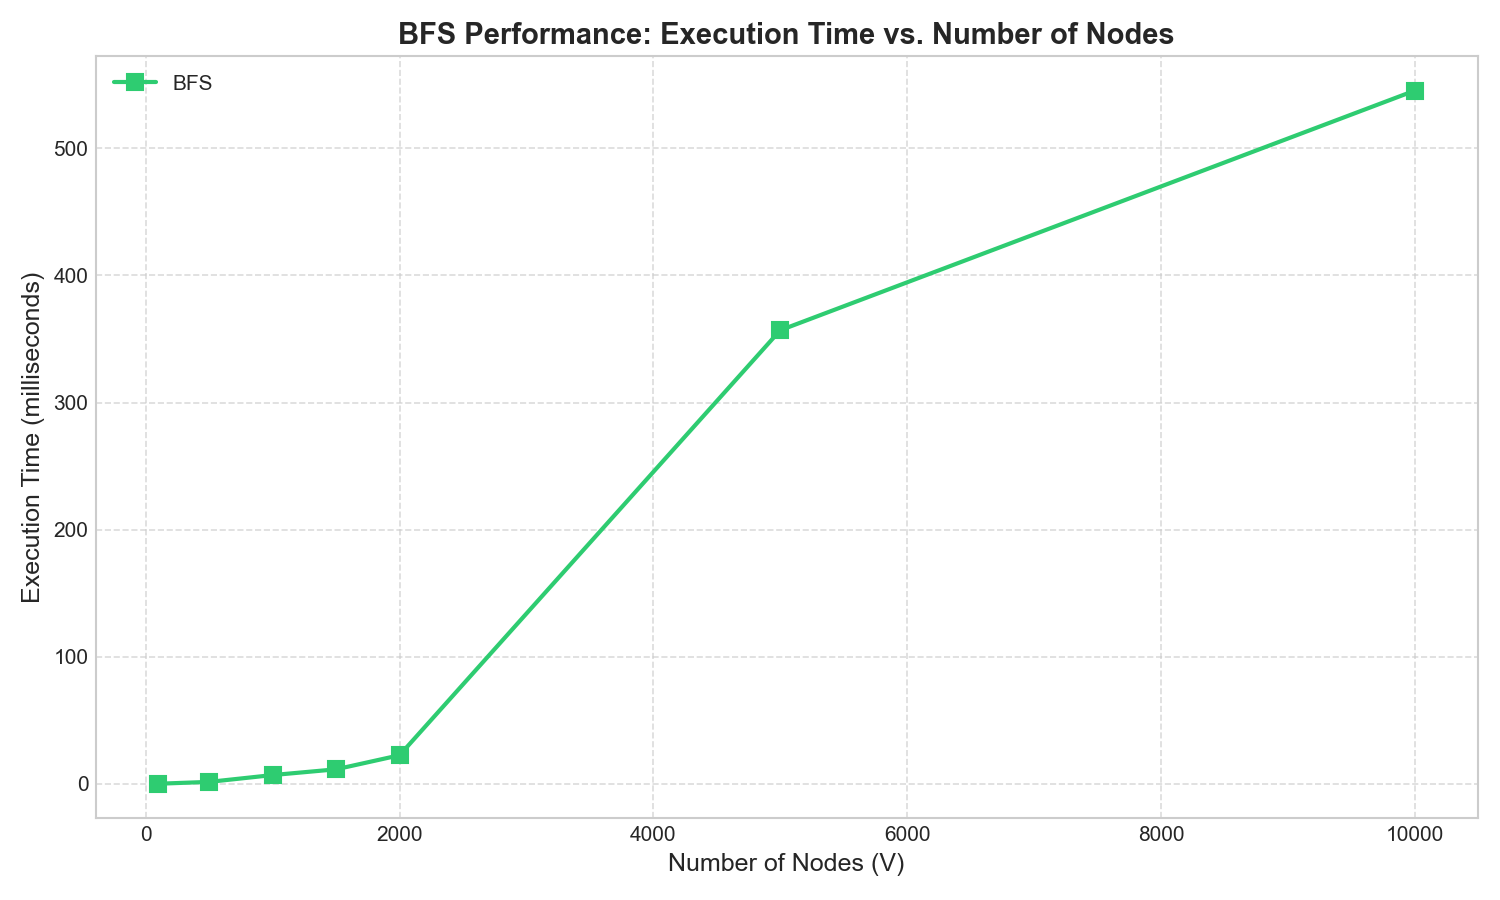
\includegraphics[width=0.83\textwidth]{../../Lab3/plots/bfs_performance_vs_nodes.png}
    \caption{BFS execution time as a function of node count}
    \label{fig:bfs-nodes}
\end{figure}

According to Figure~\ref{fig:bfs-nodes}, BFS maintains low execution times across most graph types as node count increases. The exception is the complete graph category, where the edge count grows quadratically with the number of vertices and causes a sharp rise in execution time. All other topologies produce curves that remain close to the horizontal axis at the scale shown, confirming that BFS is efficient on all but the densest structures.

The performance breakdown across all tested graph types is presented in Figure~\ref{fig:lab3-by-type}.

\begin{figure}[H]
    \centering
    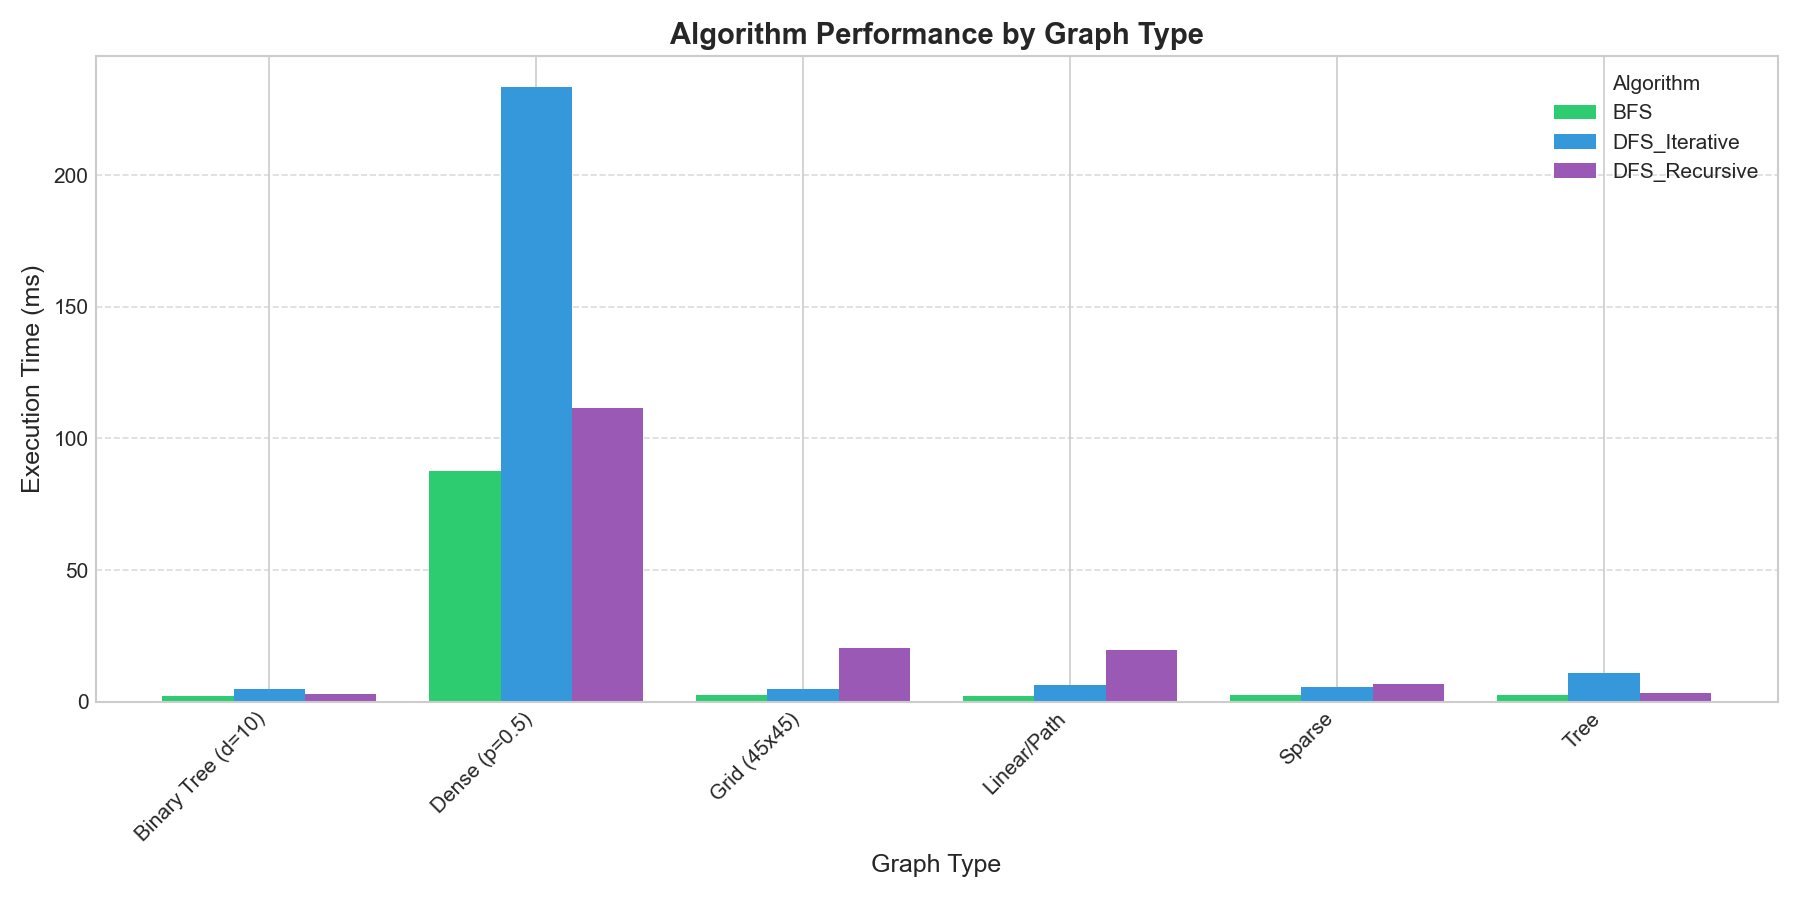
\includegraphics[width=0.88\textwidth]{../../Lab3/plots/performance_by_graph_type.png}
    \caption{DFS and BFS execution time categorized by graph topology}
    \label{fig:lab3-by-type}
\end{figure}

According to Figure~\ref{fig:lab3-by-type}, tree and grid-planar topologies impose the lowest traversal cost on both algorithms, while complete and bipartite topologies impose the highest. The complete graph is the most expensive because every vertex is connected to every other vertex, maximizing the total number of neighbor inspections. DFS consistently requires more time than BFS on complete and bipartite graphs, a pattern attributable to the larger stack depth and the greater number of repeated neighbor revisit checks before DFS completes.

\reportlabel{Conclusion}

BFS scales well on all tested graph topologies. Its deque-based optimized variant is substantially faster than the list-based base variant on graphs with large frontier layers, confirming that the \(O(1)\) vs \(O(n)\) cost of the dequeue operation is a significant practical factor. BFS is the recommended choice when memory efficiency is important and the graph is sparse or structured, because its queue size at any point is bounded by the frontier width rather than the exploration depth.

\tocsubsection{Comparative Analysis}

A direct comparison of DFS and BFS across identical inputs reveals how the two traversal strategies differ in practice. Both algorithms visit the same set of reachable vertices and both have the same theoretical time complexity, but their concrete running times and memory profiles diverge significantly depending on graph structure and density.

\reportlabel{Results}

The comparison of DFS and BFS execution time as a function of node count, aggregated across all graph types and densities, is presented in Figure~\ref{fig:dfs-vs-bfs-nodes}.

\begin{figure}[H]
    \centering
    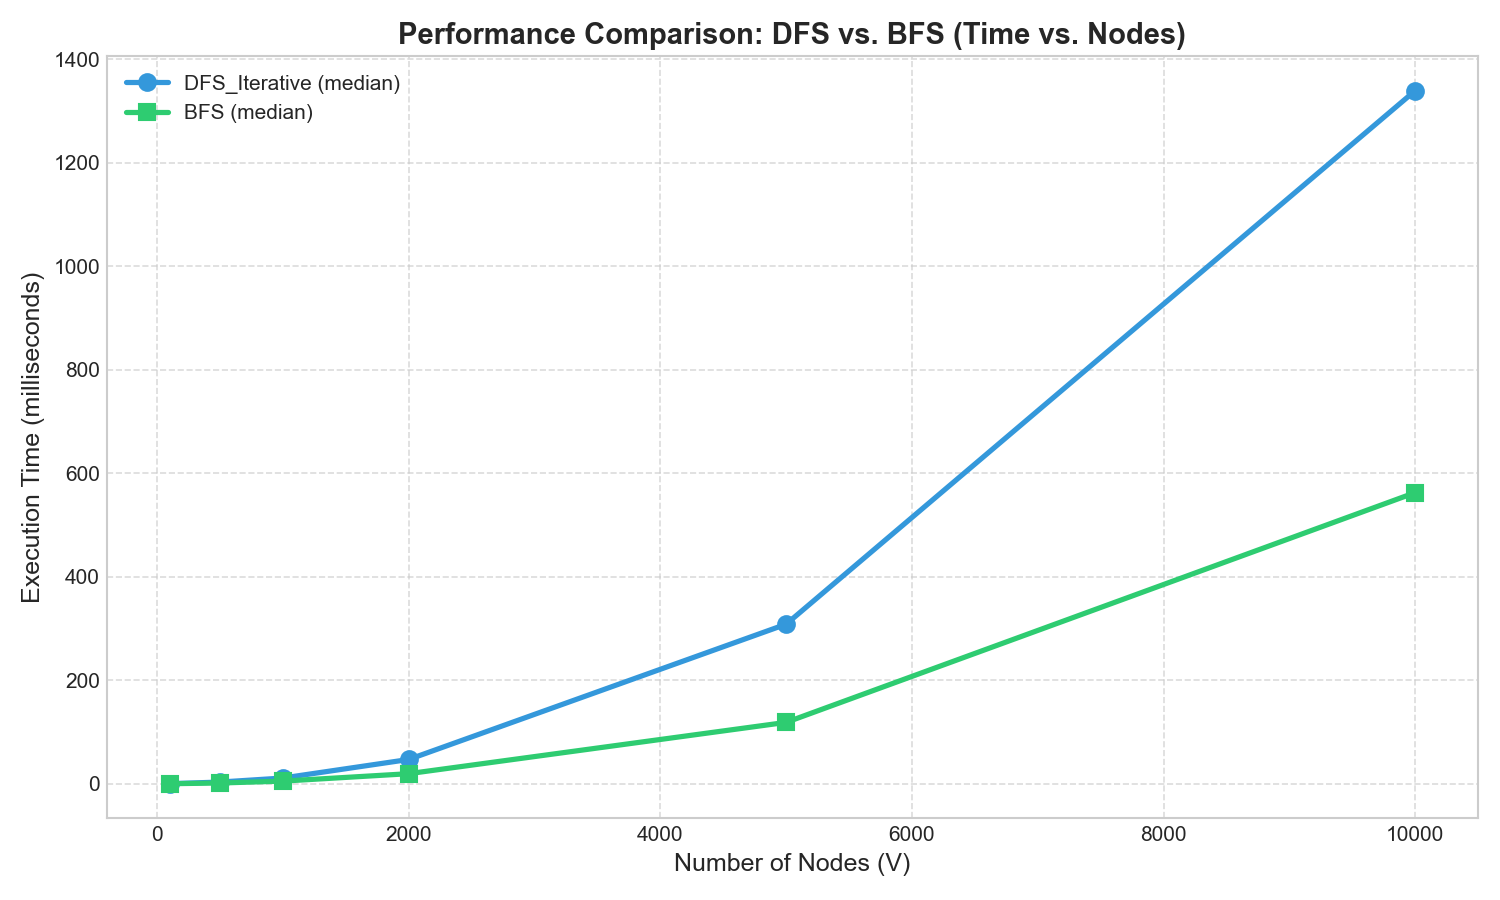
\includegraphics[width=0.88\textwidth]{../../Lab3/plots/dfs_vs_bfs_performance_nodes.png}
    \caption{DFS versus BFS execution time as a function of node count}
    \label{fig:dfs-vs-bfs-nodes}
\end{figure}

According to Figure~\ref{fig:dfs-vs-bfs-nodes}, both algorithms follow a similar growth pattern. BFS tends to perform slightly better on dense configurations while DFS and BFS are comparable on sparse inputs. The performance gap widens at higher node counts, which is consistent with the quadratic growth of edge count relative to node count under constant density.

The comparison of execution time as a function of edge count is presented in Figure~\ref{fig:dfs-vs-bfs-edges}.

\begin{figure}[H]
    \centering
    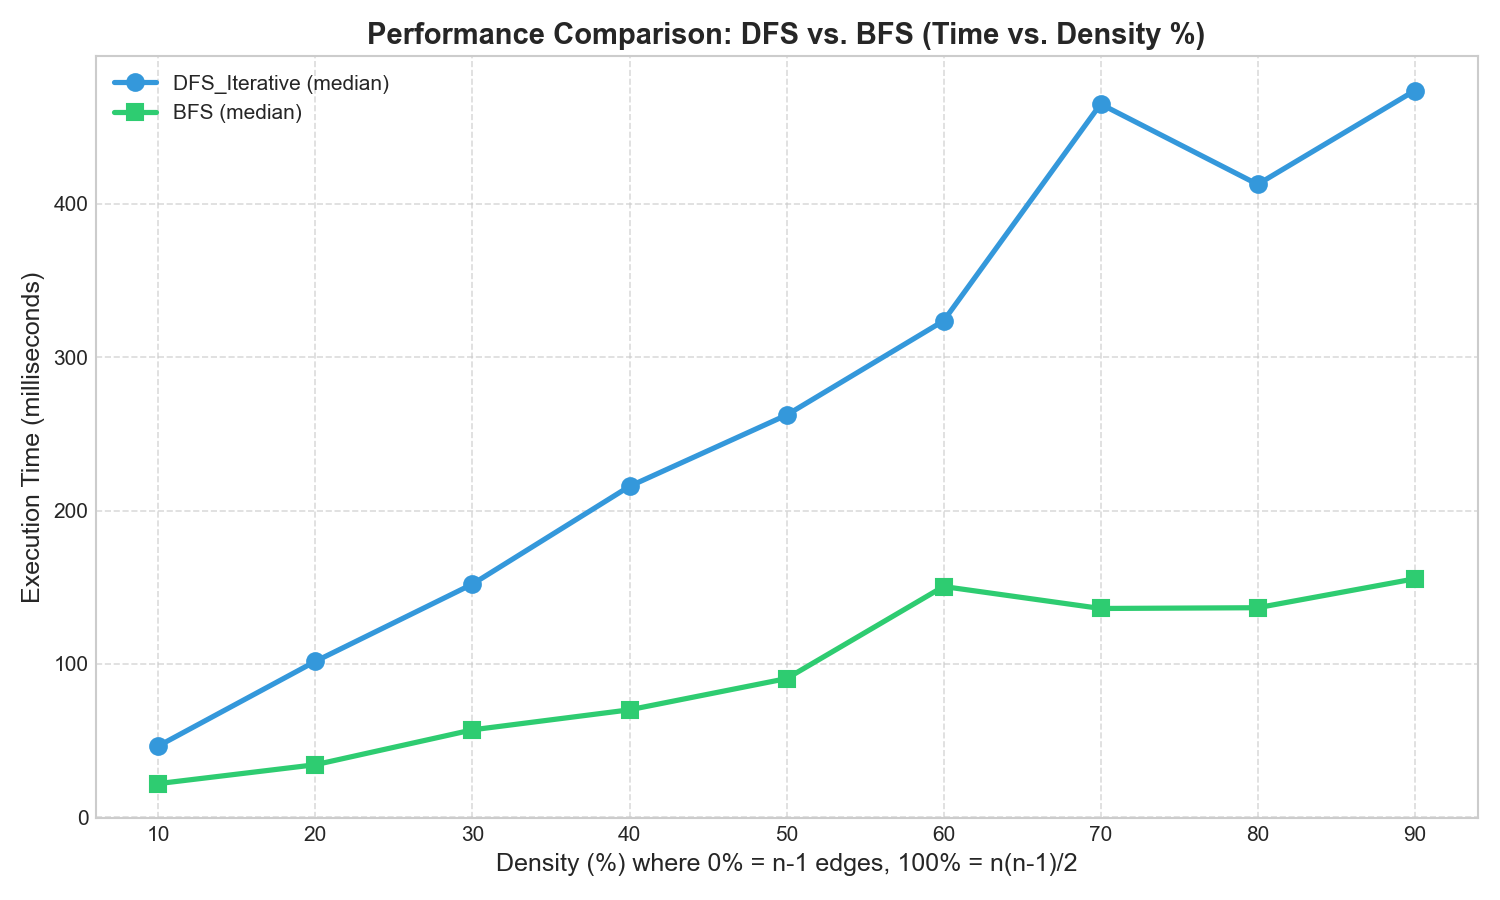
\includegraphics[width=0.88\textwidth]{../../Lab3/plots/dfs_vs_bfs_performance_edges.png}
    \caption{DFS versus BFS execution time as a function of edge count}
    \label{fig:dfs-vs-bfs-edges}
\end{figure}

According to Figure~\ref{fig:dfs-vs-bfs-edges}, edge count is a stronger predictor of running time than vertex count for both algorithms. The near-linear growth of execution time with edge count confirms that both algorithms process each edge a constant number of times, consistent with the theoretical \(O(V + E)\) bound.

The memory usage comparison is presented in Figure~\ref{fig:memory-comp}.

\begin{figure}[H]
    \centering
    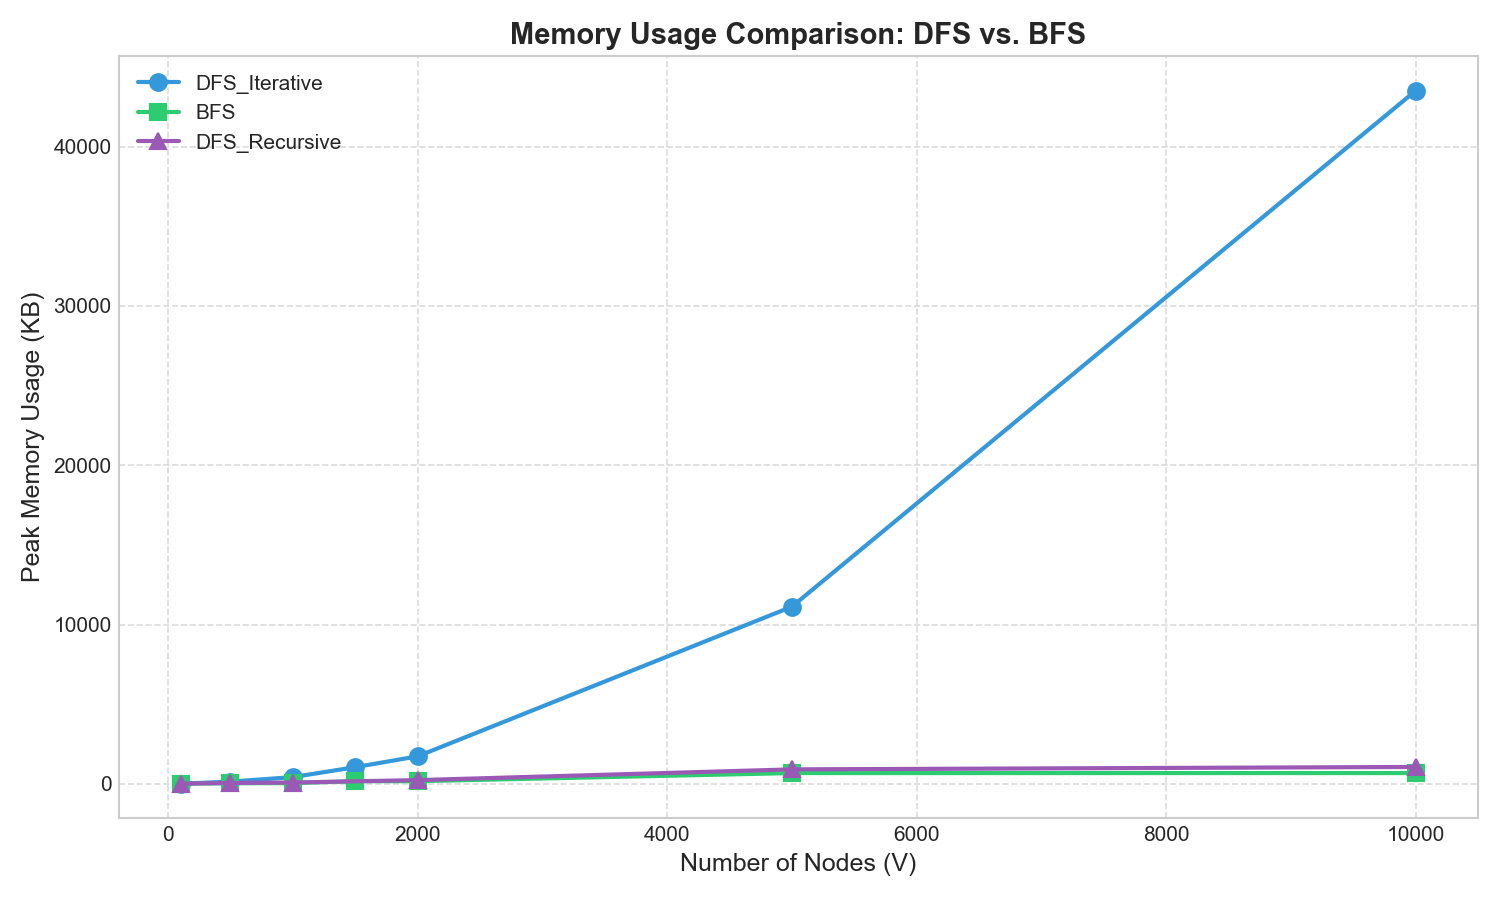
\includegraphics[width=0.88\textwidth]{../../Lab3/plots/memory_usage_comparison.png}
    \caption{Peak memory usage comparison between DFS and BFS}
    \label{fig:memory-comp}
\end{figure}

According to Figure~\ref{fig:memory-comp}, the memory behavior of the two algorithms is the most clearly differentiated result of the laboratory. DFS peak memory grows substantially on denser inputs because the stack accumulates unprocessed neighbors from multiple branches simultaneously. BFS peak memory remains comparatively low across all configurations because the queue holds only the current frontier layer.

The comprehensive four-panel analysis combining time, density, memory, and topology perspectives is presented in Figure~\ref{fig:lab3-comp}.

\begin{figure}[H]
    \centering
    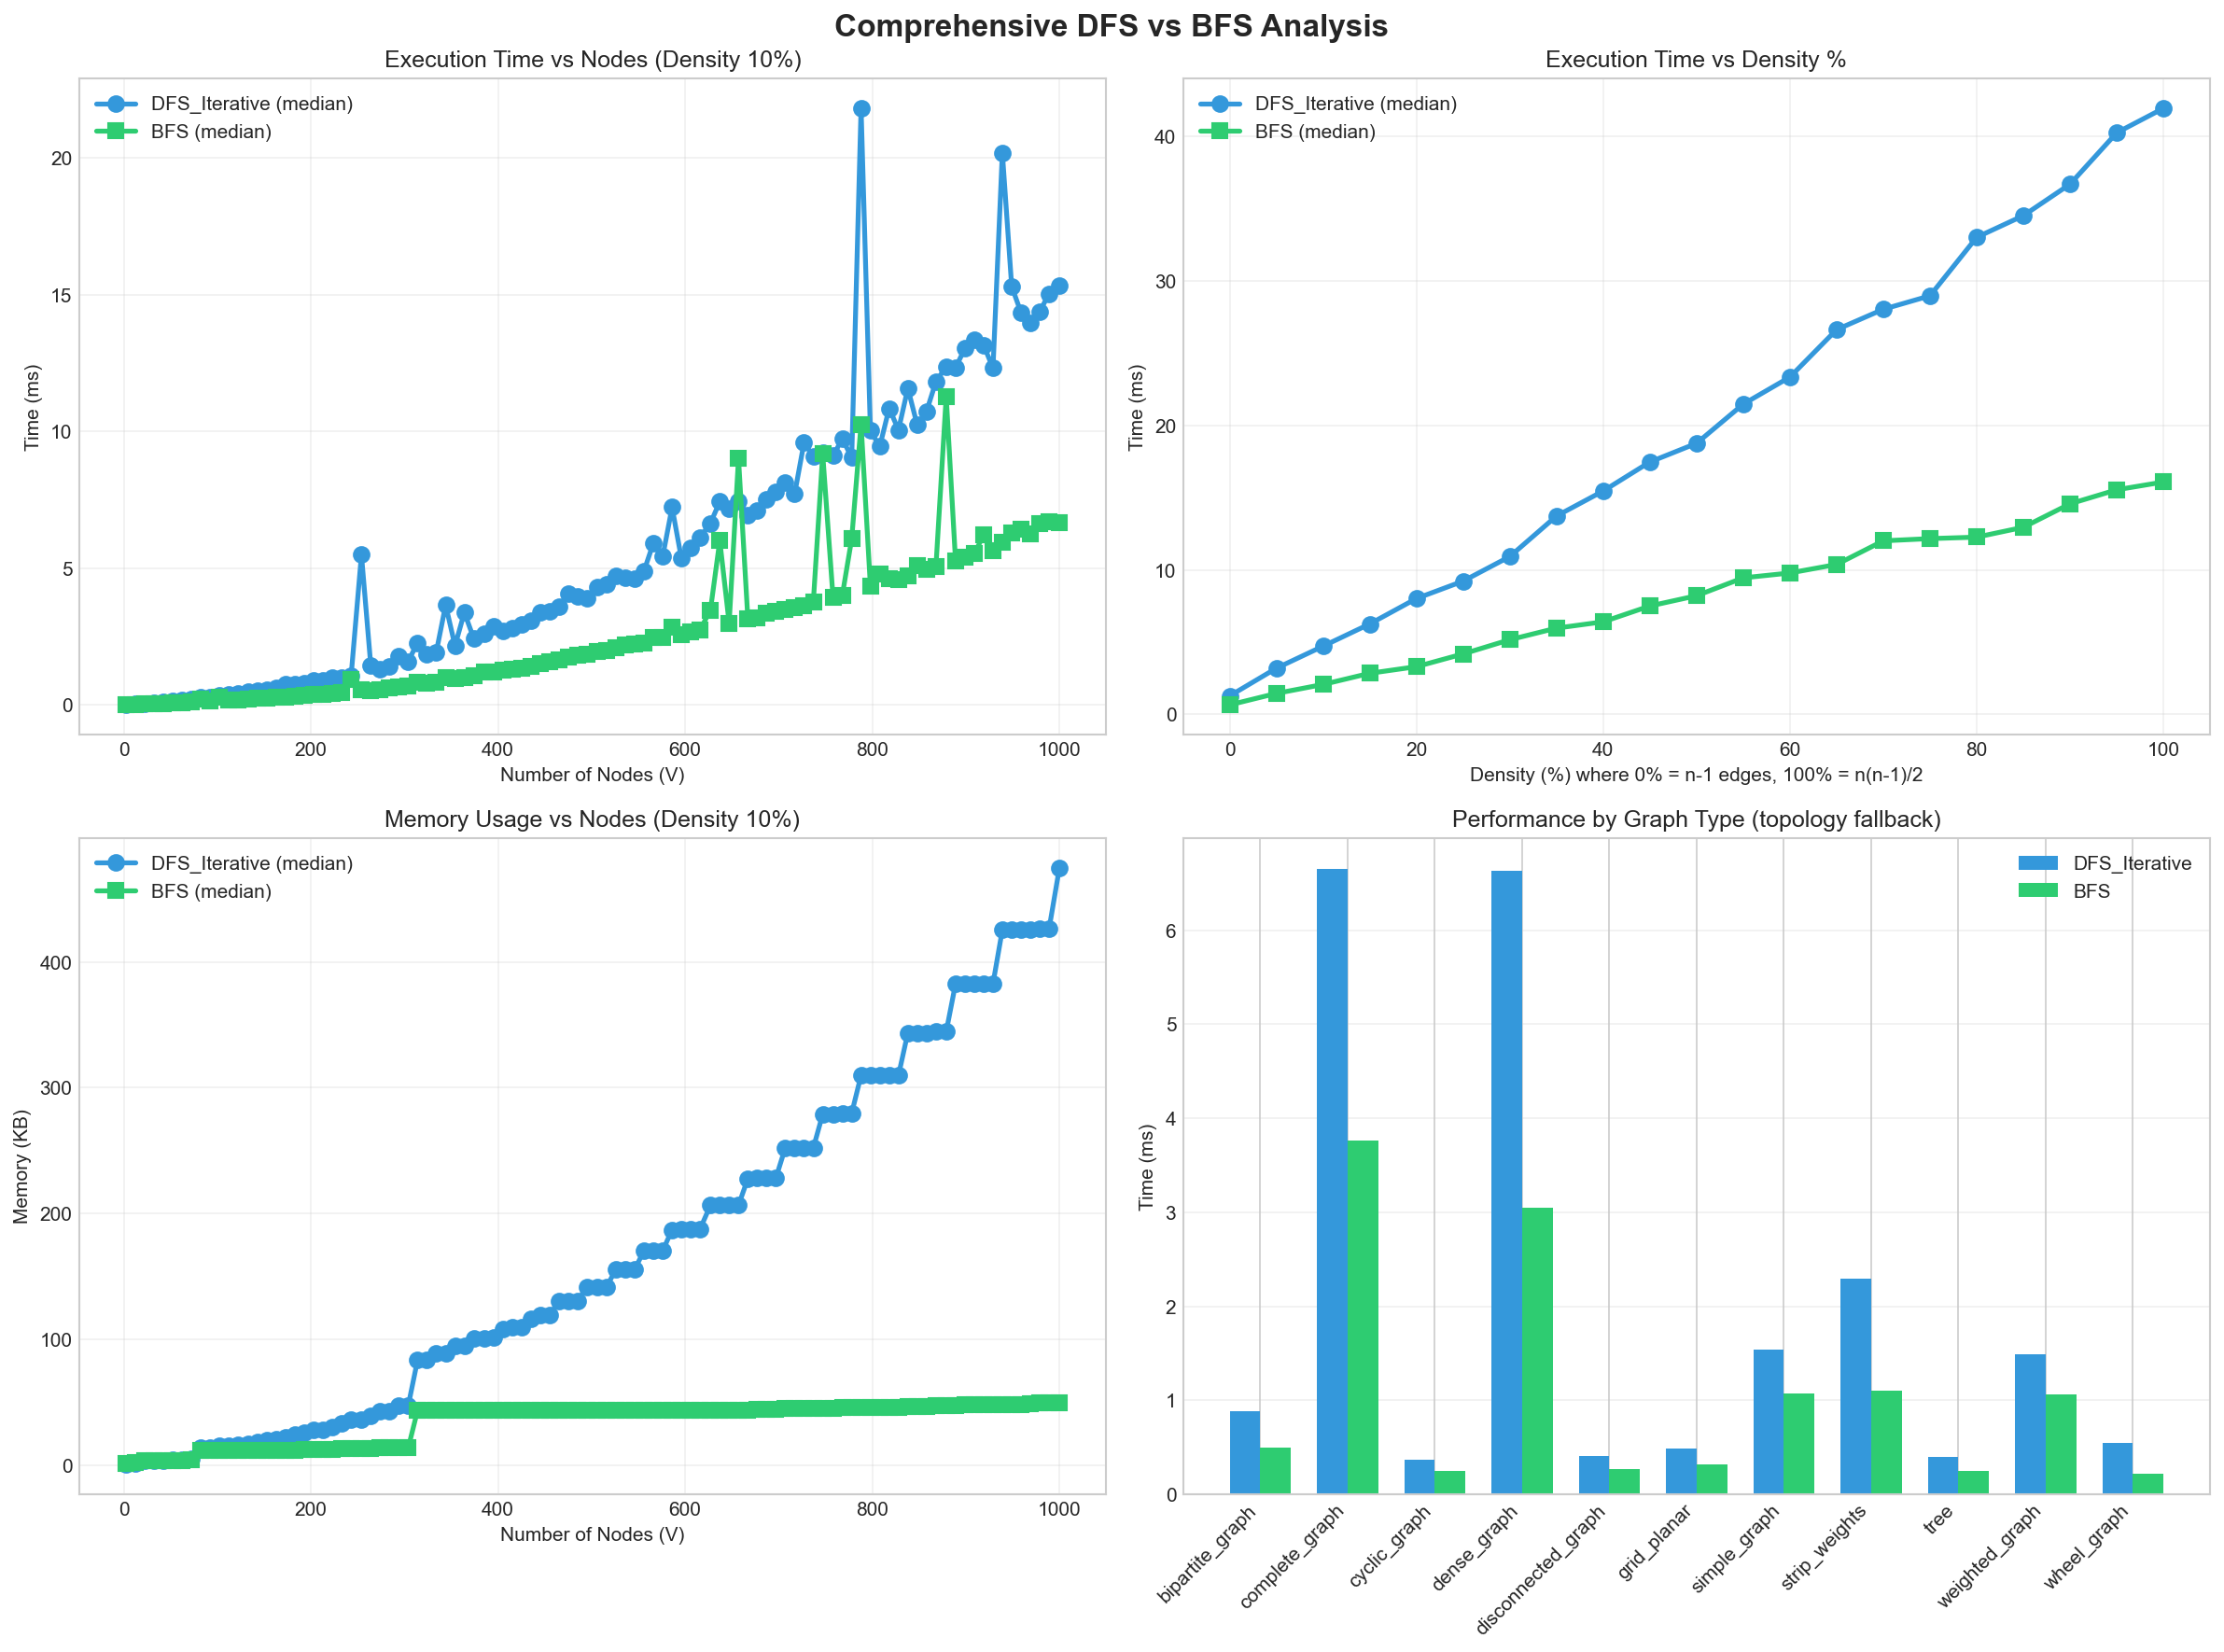
\includegraphics[width=0.90\textwidth]{../../Lab3/plots/comprehensive_analysis.png}
    \caption{Comprehensive DFS and BFS empirical analysis across all dimensions}
    \label{fig:lab3-comp}
\end{figure}

According to Figure~\ref{fig:lab3-comp}, the four-panel view confirms that BFS is the better performer from a memory perspective across all density levels. In the execution time dimension, the two algorithms are comparable on most configurations, with BFS having a slight advantage at high density. The topology panel reconfirms that tree and grid-planar structures are the least expensive for both algorithms, and that the complete graph is the most expensive.

\reportunnumberedsection{CONCLUSION}

The laboratory confirmed that both DFS and BFS follow the theoretical \(O(V + E)\) time complexity, and that the empirical results agree closely with this prediction across all tested graph sizes and densities. Both algorithms exhibit low execution times on sparse and structured topologies such as trees and grid-planar graphs, and both slow down proportionally as edge density increases. At 200 vertices and \(50\%\) fill, DFS required \(30.207\) ms and BFS required \(35.760\) ms, confirming near-identical speed at moderate density.

The primary empirical distinction between the two algorithms is their memory behavior. DFS peak memory at 200 nodes reached \(86.64\) KB while BFS required only \(4.29\) KB under the same conditions, a ratio of more than twenty to one. This difference arises from the stack-based exploration of DFS: on a dense graph, many vertices are pushed onto the stack before the traversal backtracks, while BFS limits the queue to the current level frontier. On the bipartite topology at 1000 nodes, DFS reached \(659.13\) KB compared with \(48.57\) KB for BFS, amplifying the same effect. BFS is therefore the better choice in memory-constrained environments, particularly on dense or wide graphs.

The choice of internal data structures was shown to have a decisive impact on performance. The base implementations using list-based visited checks and list-based queues are significantly slower and more memory-intensive than the optimized variants using Python \texttt{set} for visited tracking and \texttt{deque} for queue operations. The list-based \texttt{pop(0)} in the BFS base variant has \(O(n)\) cost per dequeue, which can dominate total running time on large graphs. This finding demonstrates that algorithmic complexity alone does not fully determine practical performance; the quality of the implementation is equally important.

The two-classification approach used in this laboratory, combining density-based and topology-based input generation, produced a more complete empirical picture than a single classification would have provided. The density-based benchmark isolated the effect of edge density, while the topology-based benchmark revealed how structural properties such as tree depth and bipartite structure influence memory usage. Future work could extend this study to include weighted graphs, larger vertex counts in the range of ten thousand to one hundred thousand, and a comparison of recursive versus iterative DFS to quantify the effect of Python's recursion limit on performance.

\reportreferences{
\bibitem{gfg-bfs}
GeeksforGeeks. \textit{Breadth First Search or BFS for a Graph} [online]. [cited 07.05.2026]. Available: \url{https://www.geeksforgeeks.org/breadth-first-search-or-bfs-for-a-graph/}.

\bibitem{gfg-dfs}
GeeksforGeeks. \textit{Depth First Search or DFS for a Graph} [online]. [cited 07.05.2026]. Available: \url{https://www.geeksforgeeks.org/depth-first-search-or-dfs-for-a-graph/}.

\bibitem{yt}
William Fiset. \textit{Graph Traversal Algorithms} [video online]. YouTube, 2018. [cited 07.05.2026]. Available: \url{https://www.youtube.com/watch?v=zaBhtODEL0w}.

\bibitem{repo}
Ple\c{s}u D. \textit{aa-course-repo, Lab 3 source folder} [online]. GitHub, 2026. [cited 07.05.2026]. Available: \url{https://github.com/Prince-of-Nothing/aa-course-repo/tree/main/Lab3}.
}

\end{document}
